\documentclass[aspectratio=169,13pt,fleqn,t] {beamer}
%
% Choose how your presentation looks.
%
% For more themes, color themes and font themes, see:
% http://deic.uab.es/~iblanes/beamer_gallery/index_by_theme.html
%
\mode<presentation>
{
	\usetheme{Madrid}      % 整体主题
	\usecolortheme{beaver} % 配色主题（棕红系）
	\usefonttheme{serif}   % 全局衬线字体（正文宋体类）
	\setbeamertemplate{items}[default] % 【items父模板】控制 itemize+enumerate 符号
%	\setbeamertemplate{items}{\Large\beamertemplateballitem}
	\setbeamertemplate{sections/subsections in toc}[ball] % 目录里章节用圆圈标记
	
	%  \setbeamertemplate{navigation symbols}{} % 取消注释可隐藏底部导航小图标
	\setbeamertemplate{caption}[numbered] % 图/表标题带编号：图1、表1
}
\usepackage{array,booktabs}
\usepackage[,UTF8,linespread=1.2]{ctex}
\usepackage{wrapfig}
\usepackage{caption}
\usepackage{tcolorbox}
\tcbuselibrary{skins}
\captionsetup[figure]{name=图,labelsep=period}
\usepackage{pdfpages}
\usepackage{tabularx,array}
\usetikzlibrary{arrows.meta,intersections,positioning}
\captionsetup[figure]{,aboveskip=-5pt}

\usepackage{xcolor}
\definecolor{xy_blue}{cmyk}{0.6,0.35,0.0,0.4}
\definecolor{xy_orange}{cmyk}{0.0,0.7,1.0,0.0}
\definecolor{xy_green}{cmyk}{0.2,0.0,1.0,0.15}
\xdefinecolor{xy_gold}{RGB}{135,103,79}
\xdefinecolor{xy2_gold}{cmyk}{0,0.35,0.75,0.05}

\setbeamercolor{section number projected}{fg=red,bg=red!20}%控制球的颜色
\setbeamercolor{subsection number projected}{fg=blue,bg=blue!40}
\setbeamercolor{item}{fg=xy_gold} %设置列表项颜色

\usepackage{amsthm}
\newtheorem{peroration}{结论：}
\newtheorem*{exploration}{探究：}
\newtheorem*{prooft}{证明：}
\newtheorem*{solve}{解:} 
\newtheorem{instance}{例}   % 解：独立计数器
\newtheorem*{definate}{定义：}
\newtheorem{practice}{练习}
\newtheorem{exercise}{习题}
\newtheorem{Prob}{}
     

% 配色（你前面需要的，每个环境单独颜色）
\setbeamercolor{theorem}{fg=black,bg=blue!10}
\setbeamercolor{solution}{fg=black,bg=green!10}

\BeforeBeginEnvironment{peroration}{%结论： 
	\setbeamercolor{block title}{bg=xy_green,fg=white}
	\setbeamercolor{block body}{bg=xy_green!10}
}
\AfterEndEnvironment{peroration}{
	\setbeamercolor{block title}{bg=xy_blue,fg=white}
	\setbeamercolor{block body}{bg=xy_blue!10}
}
\BeforeBeginEnvironment{exploration}{%探究
	\setbeamercolor{block title}{bg=xy_orange,fg=white}
	\setbeamercolor{block body}{bg=xy_orange!10}
}
\AfterEndEnvironment{peroration}{
	\setbeamercolor{block title}{bg=xy_blue,fg=white}
	\setbeamercolor{block body}{bg=xy_blue!10}
}
\BeforeBeginEnvironment{solution}{%解
	\begingroup
	\setbeamercolor{block title}{bg=xy_green,fg=white}
	\setbeamercolor{block body}{bg=xy_green!10}
}
\AfterEndEnvironment{solution}{
	\endgroup
}
\BeforeBeginEnvironment{prooft}{%证明
	\setbeamercolor{block title}{bg=xy_green,fg=white}
	\setbeamercolor{block body}{bg=xy_green!10}
}
\AfterEndEnvironment{prooft}{
	\setbeamercolor{block title}{bg=xy_green,fg=white}
	\setbeamercolor{block body}{bg=xy_green!10}
}
\BeforeBeginEnvironment{solve}{%解：
	\setbeamercolor{block title}{bg=xy_orange!60,fg=white}
	\setbeamercolor{block body}{bg=xy_orange!10}
}
\AfterEndEnvironment{solve}{%解：
	\setbeamercolor{block title}{bg=xy_orange!60,fg=white}
	\setbeamercolor{block body}{bg=xy_orange!10}
}
   
\BeforeBeginEnvironment{instance}{% 例子
	\begingroup
   	\setbeamercolor{block title}{bg=xy_gold!40,fg=white}
   	\setbeamercolor{block body}{bg=xy_gold!10}
   }
\AfterEndEnvironment{instance}{
	\endgroup
   }     
\BeforeBeginEnvironment{practice}{% 练习
	\begingroup
	\setbeamercolor{block title}{bg=xy_gold!40,fg=white}
	\setbeamercolor{block body}{bg=xy_gold!10}
}
\AfterEndEnvironment{practice}{
	\endgroup
}    

\BeforeBeginEnvironment{exercise}{% 习题
	\begingroup
	\setbeamercolor{block title}{bg=xy_gold!40,fg=white}
	\setbeamercolor{block body}{bg=xy_gold!10}
}
\AfterEndEnvironment{exercise}{
	\endgroup
} 

\BeforeBeginEnvironment{Prob}{% 习题
	\begingroup
	\setbeamercolor{block title}{bg=xy_gold!40,fg=white}
	\setbeamercolor{block body}{bg=xy_gold!10}
}
\AfterEndEnvironment{Prob}{
	\endgroup
} 
   
\renewcommand{\thefigure}{\arabic{figure}}

\title[P57复习参考题2答案解析]{P57复习参考题2答案解析}
\author[好好学习，努力向上]{}
\institute{}
\date{2026.9.30}
\setbeamertemplate{theorems}[numbered]

\AtBeginSection[]
{
  \begin{frame}<beamer>
    \frametitle{本节主要内容}
    \tableofcontents[currentsection,currentsubsection]
  \end{frame}
}

\AtBeginDocument{
	\setlength{\abovedisplayskip}{3pt}
	\setlength{\belowdisplayskip}{3pt}
	}


\begin{document}
\begin{frame}{}
	\titlepage
\end{frame}

%\begin{frame}{内容概览}
%	\tableofcontents
%\end{frame}

\begin{frame}
	\vspace{-1em}
	\begin{Prob}
		某夏令营有 $48$ 人，出发前要从 A，B 两种型号的帐篷中选择一种。A 型号的帐篷比 B 型号的少 $5$ 顶。若只选 A 型号的，每顶帐篷住 $4$ 人，则帐篷不够；每顶帐篷住 $5$ 人，则有一顶帐篷没有住满。若只选 B 型号的，每顶帐篷住 $3$ 人，则帐篷不够；每顶帐篷住 $4$ 人，则有帐篷多余。设 A 型号的帐篷有 $x$ 顶，用不等式将题目中的不等关系表示出来。
	\end{Prob}
	\vspace{-1em}
	\begin{solve}
		\small
		设 A 型号帐篷有 $x$ 顶，则 B 型号帐篷有 $(x+5)$ 顶，则
		\vspace{-1em}
		\[
		\begin{cases}
			x>0,\ x\in \mathbf{N}^*,\\
			x+5>0,\\
			4x<48,\\
			0\leq 5x-48<5,\\
			3(x+5)<48,\\
			4(x+5)>48,
		\end{cases}
		\]
		
		\vspace{-1em}
		解得 $9\leq x<11$。
	\end{solve}
\end{frame}

\begin{frame}
	\begin{Prob}
		用不等式“$>$”或“$<$”填空：
		\begin{enumerate}[(1)]
		\item  若 $a>b$，且 $\dfrac{1}{a}>\dfrac{1}{b}$，则 $ab$ \underline{\hspace{2.5em}} $0$；
		
		\item  若 $c>a>b>0$，则 $\dfrac{a}{c-a}$ \underline{\hspace{2.5em}} $\dfrac{b}{c-b}$；
		
		\item  若 $a>b>c>0$，则 $\dfrac{a}{b}$ \underline{\hspace{2.5em}} $\dfrac{a+c}{b+c}$。
	\end{enumerate}
	\end{Prob}
	\vspace{-1em}
	\begin{solve}
		\textbf {答案：}
		
		$(1)$ $<$ \quad $(2)$ $>$ \quad $(3)$ $>$
		\begin{enumerate}[(1)]
			\item  解析：$\dfrac{1}{a}-\dfrac{1}{b}=\dfrac{b-a}{ab}>0$。因为 $a>b>0$，所以 $a>0$，$b>0$，$a-b>0$，所以 $\dfrac{b-a}{ab}<0$，即 $\dfrac{1}{a}<\dfrac{1}{b}$。
		\end{enumerate}
	\end{solve}
\end{frame}

\begin{frame}{}
	\begin{solve}
		\begin{enumerate}[(1)]
			\setcounter{enumi}{1}
			\item 解法一：$\dfrac{a}{c-a}-\dfrac{b}{c-b}=\dfrac{ac-bc+ab-bc}{(c-a)(c-b)}=\dfrac{(a-b)c}{(c-a)(c-b)}$。因为 $c>a>b>0$，所以 $c-a>0$，$c-b>0$，$a-b>0$，所以 $\dfrac{(a-b)c}{(c-a)(c-b)}>0$，即 $\dfrac{a}{c-a}>\dfrac{b}{c-b}$。
			
			解法二：因为 $c>a>b>0$，所以 $c-b>c-a>0$，所以 $\dfrac{1}{c-a}>\dfrac{1}{c-b}>0$，又 $a>b>0$，所以 $\dfrac{a}{c-a}>\dfrac{b}{c-b}$。
			\item $\dfrac{a}{b}-\dfrac{a+c}{b+c}=\dfrac{ab+ac-ab-bc}{b(b+c)}=\dfrac{(a-b)c}{b(b+c)}$。因为 $a>b>c>0$，所以 $a-b>0$，$b+c>0$，所以 $\dfrac{(a-b)c}{b(b+c)}>0$，即 $\dfrac{a}{b}>\dfrac{a+c}{b+c}$。
		\end{enumerate}
	\end{solve}
\end{frame}

\begin{frame}
	\begin{Prob}
		\begin{enumerate}[(1)]
			\item 在面积为定值 $S$ 的扇形中，半径是多少时扇形的周长最小？
			\item 在周长为定值 $P$ 的扇形中，半径是多少时扇形的面积最大？
		\end{enumerate}
	\end{Prob}
	
	\begin{solve}
		\begin{enumerate}[(1)]
			\item 设弧长为 $l$，半径为 $R$，则 $\dfrac{1}{2}lR=S$，周长 $y=2R+l\geq 2\sqrt{2Rl}=2\sqrt{4S}=4\sqrt{S}$，当且仅当 $2R=l$，即 $R=\sqrt{S}$ 时，等号成立，此时周长最小，为 $4\sqrt{S}$。
			\item 设弧长为 $l$，半径为 $R$，则 $2R+l=P$，面积 $S=\dfrac{1}{2}lR=\dfrac{1}{2}R(P-2R)=R\left(\dfrac{1}{2}P-R\right) \leqslant\left(\dfrac{\frac{p}{2}-R+R}{2}\right)=\dfrac{P^2}{16}$，
			
			当且仅当 $R=\dfrac{1}{2}P - R$，即 $R=\dfrac{P}{4}$ 时，等号成立，此时面积最大，为 $\dfrac{P^2}{16}$。
		\end{enumerate}
		
	\end{solve}
\end{frame}

\begin{frame}
	\vspace{-1em}
	\begin{Prob}
		求下列不等式的解集：
		\begin{enumerate}[(1)]
			\item $14-4x^2\geq x$；
			\item  $x^2-14x+45\leq 0$；
			\item   $x^2+6x+10>0$；
			\item   $x(x+2)>x(3-x)+1$。
		\end{enumerate}		
	\end{Prob}
	\vspace{-1em}
	\begin{solve}
		\begin{enumerate}[(1)]
		
	\item  $\left\{x\;\middle|\;-2\leq x\leq \dfrac{7}{4}\right\}$
	
	\item  $\{x\mid 5\leq x\leq 9\}$
	
	\item  $\mathbf{R}$
	
	\item  $\left\{x\;\middle|\;x<-\dfrac{1}{2}\ \text{或}\ x>1\right\}$
	\end{enumerate}
	\end{solve}
\end{frame}

\begin{frame}
	\begin{Prob}
	若 $a,\ b>0$，且 $ab=a+b+3$，求 $ab$ 的取值范围。
	\end{Prob}
	
	\begin{solve}
		因为 $a,b>0$，所以 $ab-3=a+b\geq 2\sqrt{ab}$，
		
		所以 $ab-2\sqrt{ab}-3\geq 0$，即 \;$(\sqrt{ab})^2 - 2\sqrt{ab}- 3 \geq 0$，
		
		所以 $\sqrt{ab}\leq -1$（舍去）或 $\sqrt{ab}\geq 3$，
		
		所以 $ab\geq 9$，当且仅当 $a=b=3$ 时等号成立，
		
		所以 $ab$ 的取值范围是 $ab\geq 9$。
		
	\end{solve}
\end{frame}

\begin{frame}
	\begin{Prob}
		当 $k$ 取什么值时，一元二次不等式 $2kx^2+kx-\dfrac{3}{8}<0$ 对一切实数 $x$ 都成立？
	\end{Prob}
	
	\begin{solve}
		由题意可得 $k\neq 0$，$2kx^2+kx-\dfrac{3}{8}<0$ 对一切实数 $x$ 都成立，
		
		所以 $k<0$，且对于方程 $2kx^2+kx-\dfrac{3}{8}=0$，$\Delta=k^2-4\cdot 2k\left(-\dfrac{3}{8}\right)<0$，
		
		解得 $-3<k<0$。
		
		综上所述，$k$ 的取值范围是 $-3<k<0$。
		
	\end{solve}
\end{frame}

\begin{frame}
	\vspace{-1em}
	\begin{Prob}\small
	一般认为，民用住宅的窗户面积必须小于地板面积，但窗户面积与地板面积的比应不小于 $10\%$，而且这个比值越大，采光效果越好。	
	\begin{enumerate}[(1)]
		\item 若一所公寓窗户面积与地板面积的总和为 $220$ m$^2$，则这所公寓的窗户面积至少为多少平方米？
		\item 若同时增加相同的窗户面积和地板面积，公寓的采光效果是变好了还是变坏了？
	\end{enumerate}
	\end{Prob}
	\vspace{-1em}
	\begin{solve}

				(1) 设窗户面积为 $x$ m$^2$，则地板面积为 $(220-x)$ m$^2$。由题意可得
				\[
				\begin{cases}
					x<220-x,\\
					\dfrac{x}{220-x}\geq 10\%,\\
					x>0,\\
					220-x>0,
				\end{cases}
				\]
				解得 $20\leq x<110$，所以窗户面积至少为 $20$ $ \mathrm{m^2}$。	
\end{solve}
\end{frame}
	
	

\begin{frame}
	\begin{solve}[接上页]	
	\vspace{1ex}
	(2) 公寓的采光效果变好了。设公寓原来的窗户面积和地板面积分别为 $x,y$（$x>0,y>0,x<y$），增加的面积为 $m$ $ \mathrm{m^2}$，
	
	由题意可得 $\dfrac{x+m}{y+m}-\dfrac{x}{y}=\dfrac{m(y-x)}{(y+m)y}>0$，\rule[15pt]{0pt}{10pt}\rule[-20pt]{0pt}{10pt}
	
	即增加 $m$ $ \mathrm{m^2}$ 之后，比值变大了，故采光效果变好了。
	\end{solve}
\end{frame}

\begin{frame}
	\vspace{-1em}
	\begin{Prob}

	相等关系和不等关系之间具有对应关系：即只要将一个相等关系的命题中的等号改为不等号就可得到一个相应的不等关系的命题。请你用类比的方法探索相等关系和不等关系的对应性质，仿照下表列出尽可能多的有关对应关系的命题；指出所列的对应不等关系的命题是否正确，并说明理由。
	
	\begin{center}
		\begin{tabular}{|c|c|c|}
			\hline
		相等关系	&	\multicolumn{2}{c|}{不等关系}   \\
			\hline
			相等关系的命题 & 不等关系的命题 & 判断正误 \\
			\hline
		\upshape	(1) 若 $x=y$，则 $x^3=y^3$ & \upshape (1) 若 $x>y$，则 $x^3>y^3$ & 正确 \\
			\hline
			& & \\
			& & \\
			& & \\
			\hline
		\end{tabular}
	\end{center}
	\end{Prob}


\end{frame}

\begin{frame}{}
	\begin{solve}
			\begin{center}\upshape
			\begin{tabular}{lll}
				\toprule
				\textbf{相等关系} & \textbf{不等关系} & \textbf{判断正误} \\
				\midrule
				(1) 若 $x=y$，则 $x^3=y^3$ & (1) 若 $x>y$，则 $x^3>y^3$ & 正确 \\
				(2) 若 $x=y$，则 $|x|=|y|$ & (2) 若 $x>y$，则 $|x|>|y|$ & 错误 \\
				(3) 若 $x=y$，则 $x^2=y^2$ & (3) 若 $x>y$，则 $x^2>y^2$ & 错误 \\
				(4) 若 $x=y\neq 0$，则 $\dfrac{1}{x}=\dfrac{1}{y}$ & (4) 若 $x>y>0$，则 $\dfrac{1}{x}>\dfrac{1}{y}$ & 错误 \\
				\bottomrule
			\end{tabular}
		\end{center}
	\end{solve}
\end{frame}

\begin{frame}{}
	\begin{Prob}
		如图，居民小区要建一座八边形的休闲场所，它的主体造型平面图是由两个相同的矩形 $ABCD$ 和 $EFGH$ 构成的面积为 $200$ $\mathrm{m^2}$ 的十字形地域。计划在正方形 $MNPQ$ 上建一座花坛，造价为 $4200$ 元/$\mathrm{m^2}$；在四个相同的矩形（图中阴影部分）上铺花岗岩地坪，造价为 $210$ 元/m$^2$；再在四个空角（图中四个三角形）上铺草坪，造价为 $80$ 元/$\mathrm{m^2}$。设总造价为 $S$（单位：元），$AD$ 长为 $x$（单位：$\mathrm{m}$）。当 $x$ 为何值时，$S$ 最小？并求出这个最小值。
	\end{Prob}
	\begin{figure}
		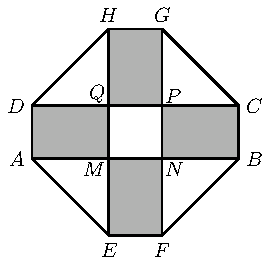
\includegraphics{Figures/budengshi2-3-3.pdf}
	\end{figure}
	
\end{frame}
\begin{frame}{}
\begin{solve}
	设 $AM=y$ $\mathrm{m}$，则 $x^2+4xy=200$，从而 $y=\dfrac{200-x^2}{4x}$。于是
	\[
	S=4\cdot 200x^2+210\times 4xy+80\times 2y^2
	\]
	\[
	=4\cdot 200x^2+210\times 4x\cdot \frac{200-x^2}{4x}+80\times 2\left(\frac{200-x^2}{4x}\right)^2
	\]
	\[
	=38000+4000x^2+\frac{400000}{x^2}\geq 38000+2\sqrt{4000x^2\cdot \frac{400000}{x^2}}=118000,
	\]
	当且仅当 $4000x^2=\dfrac{400000}{x^2}$，即 $x=\sqrt{10}$（$x=-\sqrt{10}$ 舍去）时等号成立。由上述可知，当 $AD=\sqrt{10}$ $\mathrm{m}$ 时，休闲广场总造价 $S$ 取最小值，为 $118000$ 元。
\end{solve}
\end{frame}
\begin{frame}{}
	\begin{Prob}
		购买同一种物品，可以用两种不同的策略，第一种是不考虑物品价格的升降，每次购买这种物品的数量一定；第二种是不考虑物品价格的升降，每次购买这种物品所花的钱数一定。哪种购物方式比较经济？你能把所得结论作一些推广吗？
	\end{Prob}
	\begin{solve}
			按第一种策略购物，设第一次购物时价格为 $P_1$ 元，购 $n$ kg，第二次购物时价格为 $P_2$ 元，仍购 $n$ kg（$P_1>0,P_2>0,n>0$），两次购物的平均价格为 $\dfrac{P_1n+P_2n}{2n}=\dfrac{P_1+P_2}{2}$；若按第二种策略购物，第一次花 $m$ 元，能购 $\dfrac{m}{P_1}$ kg 物品，第二次仍花 $m$ 元，能购 $\dfrac{m}{P_2}$ kg 物品，两次购物的平均价格为 $\dfrac{2m}{\dfrac{m}{P_1}+\dfrac{m}{P_2}}=\dfrac{2P_1P_2}{P_1+P_2}$。
		
		比较两次购物的平均价格。
		
		
	\end{solve}
\end{frame}
\begin{frame}{}
	\begin{solve}[接上页]
		解法一：
		\[
		\frac{P_1+P_2}{2}-\frac{2P_1P_2}{P_1+P_2}
		=\frac{(P_1+P_2)^2-4P_1P_2}{2(P_1+P_2)}
		=\frac{(P_1-P_2)^2}{2(P_1+P_2)}\geq 0,
		\]
		所以 $\dfrac{P_1+P_2}{2}\geq \dfrac{2P_1P_2}{P_1+P_2}$，当且仅当 $P_1=P_2$ 时等号成立。
		
		解法二：
		\[
		\frac{2P_1P_2}{P_1+P_2}\leq \frac{2P_1P_2}{2\sqrt{P_1P_2}}=\sqrt{P_1P_2}\leq \frac{P_1+P_2}{2},
		\]
		当且仅当 $P_1=P_2$ 时等号成立。
		
		所以用第二种购物策略比较经济。
		
		一般地，如果 $n$ 次购买同一种物品，用第二种策略购买比较经济。
	\end{solve}
\end{frame}
\end{document}
